\subsection{きなこチーム}


\subsubsection{概要}
% これこれ作った▶自己位置推定とナビゲーションは〜▶以前〜▶詳細
きなこチームは、3D-LiDARを用いた自己位置推定のロバスト性を高めるパッケージを作成した。
自己位置推定とナビゲーションはそれぞれemcl2、Nav2を使用した。
以前、人や車などの動的な障害物により自己位置推定が破綻するという問題が起きた。
その対策として、動的障害物の無い2m以上を観測することで対処していた。
3Dマップと3D-LiDARの点群を全て2次元に投影してナビゲーションを行っていた。
% しかし、3次元の異なる高さにある物体が2次元平面に投影されることで同一の物体のように扱われてしまう。
しかし、場所によって特徴がある高さが違うため、全てを圧縮するとマップの細かな情報が保持できない。
その結果、自己位置推定が非常に不安定になり、破綻することもあった。

これに対処するため、ロボットの位置によって自己位置推定器が参照するマップと点群データの高さを変化させるパッケージを作成した。


\subsubsection{開発したシステム}
3D-LiDARから2つの2次元点群データを生成するパッケージ(map\_manager)、自己位置推定で参照するマップを切り替えるパッケージ(pointcloud\_to\_dual\_scan)を開発した。
自己位置推定のために高いところをみると、ロボットが障害物を検知できない。そのため、障害物回避用、自己位置推定用の2つの点群データを生成することにした。
また、自己位置推定で参照する点群とマップは同じ高さとなっている。
\begin{itemize}
  \item \textbf{map\_manager}
    \begin{itemize}
      \item 高さ別に作成したマップを複数保持
      \item 指定した範囲にロボットが入ると、指定されたマップと指定された高さパラメータを提供
    \end{itemize}
  \item \textbf{pointcloud\_to\_dual\_scan}
    \begin{itemize}
      \item 3D-LiDARから取得した点群データを2つの2次元スキャンデータに生成して提供
      \item map\_managerから高さパラメータを受け取り、生成するデータの範囲を変更
    \end{itemize}
\end{itemize}
高さをどう切り替えているか
マップの作成方法は?
高いところだけ見れば?
パッケージごとに段落分けて説明
パッケージの相互関係



% それぞれをemcl2、Nav2に送る。
% map_managerはemcl2から送られる自己位置を受け取り、事前に指定された範囲に入ったらマップとLiDARの見る高さを指定するパラメータを発行する。
% それぞれemcl2、pointcloud_to_dual_scanが受け取る。

% \begin{figure}[h]
%   \begin{center}
%     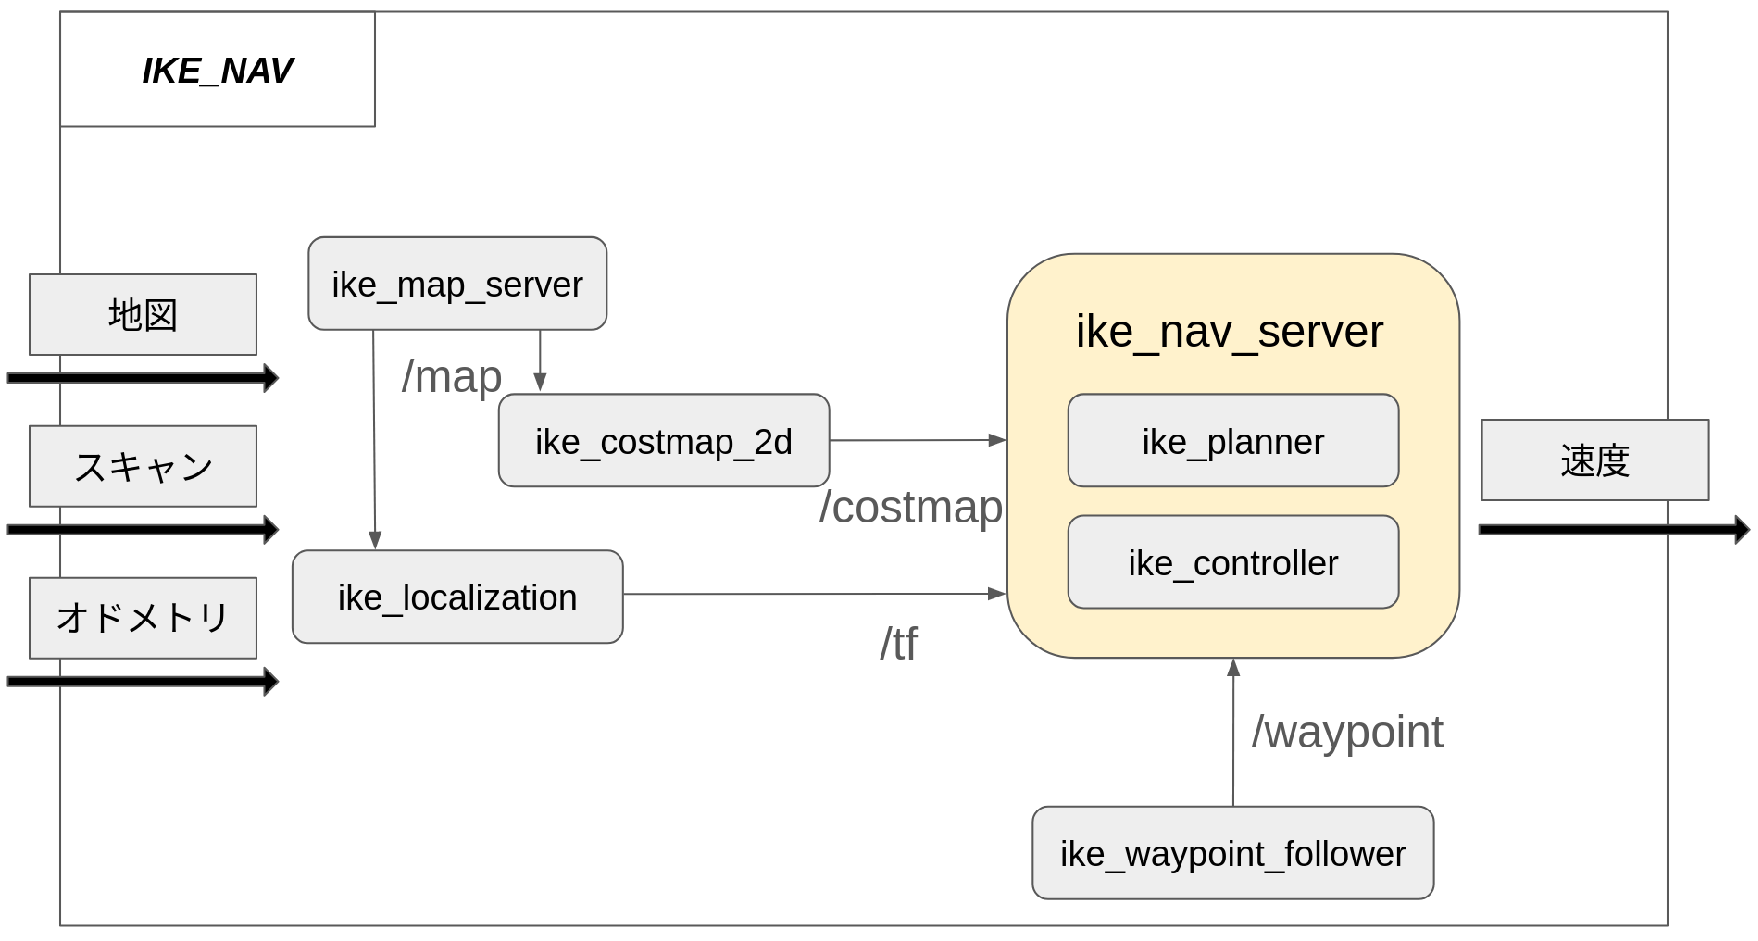
\includegraphics[width=1.0\linewidth]{figs/ike_nav.pdf}
%     \caption{ツナチームのシステム構成}
%     \label{fig:tuna_system}
%   \end{center}
% \end{figure}